\documentclass[spanish]{beamer}
\usetheme{metropolis}

%%% CODIFICACIÓN

%\usepackage[x11names, rgb, html]{xcolor}
\usepackage[spanish]{babel}
\usepackage{graphics,tikz}

%%% FUENTES

\usepackage{mathspec}
\setmainfont[
	Path=./../fuentes/, 
	UprightFont=* Regular, 
	ItalicFont=* Italic,
	BoldFont=* Bold,
  	BoldItalicFont=* Bold Italic,
]{Concourse T3}
\setmathsfont(Digits,Latin,Greek)[
	Path=./../fuentes/, 
	UprightFont=* Regular, 
	ItalicFont=* Italic,
	BoldFont=* Bold,
  	BoldItalicFont=* Bold Italic,
]{Concourse T3}
\setsansfont[
	Path=./../fuentes/, 
	UprightFont=* Regular, 
	ItalicFont=* Italic,
	BoldFont=* Bold,
  	BoldItalicFont=* Bold Italic,
]{Concourse T3}
\setmonofont[
  Path=./../fuentes/, 
  UprightFont=* Regular,% 
  %ItalicFont=* Italic,
  BoldFont=* Bold,
    %BoldItalicFont=* Bold Italic,
    SizeFeatures={Size=8},
]{FiraCode}

%\setbeamertemplate{navigation symbols}{}

%%% COLORES

%% Colores de Solarized

\definecolor{sbase03}{HTML}{002B36}
\definecolor{sbase02}{HTML}{073642}
\definecolor{sbase01}{HTML}{586E75}
\definecolor{sbase00}{HTML}{657B83}
\definecolor{sbase0}{HTML}{839496}
\definecolor{sbase1}{HTML}{93A1A1}
\definecolor{sbase2}{HTML}{EEE8D5}
\definecolor{sbase3}{HTML}{FDF6E3}
\definecolor{syellow}{HTML}{B58900}
\definecolor{sorange}{HTML}{CB4B16}
\definecolor{sred}{HTML}{DC322F}
\definecolor{smagenta}{HTML}{D33682}
\definecolor{sviolet}{HTML}{6C71C4}
\definecolor{sblue}{HTML}{268BD2}
\definecolor{scyan}{HTML}{2AA198}
\definecolor{sgreen}{HTML}{859900}

%% Colores del documento

\definecolor{background}{RGB}{237,237,237}
\definecolor{text}{RGB}{78,78,78}
\definecolor{accent}{RGB}{129, 26, 24}
\definecolor{accent2}{HTML}{814918}
\definecolor{accent3}{HTML}{136618}
\definecolor{accent4}{HTML}{0F4B4E}
\definecolor{accent5}{HTML}{681341}
\definecolor{accent6}{HTML}{1F1B5A}

%%% LISTINGS

%\usepackage{listingsutf8}
\usepackage{listings-golang}

%% Las tildes

\lstset{
  inputencoding=utf8/latin1
}

%% Colores de Solarized para listings

\lstset{
  basicstyle=\scriptsize\ttfamily,%
  breaklines=true,%
  captionpos=b,                    % sets the caption-position to bottom
  tabsize=2,                     % sets default tabsize to 2 spaces
  %keywordstyle=\color{red},
}

\setbeamerfont{framesubtitle}{size=\normalfont\tiny}
\setbeamercolor{framesubtitle}{fg=white}


%%% AJUSTES DE BEAMER

% ¿Negrita en el título de diapositiva o no?
%\setbeamertemplate{frametitle}{\color{accent}\vspace*{1cm}\bfseries\insertframetitle\par\vskip-6pt}

%\setbeamertemplate{frametitle}{\color{accent4}\vspace*{1cm}\insertframetitle\par\vskip-6pt}

\setbeamertemplate{itemize items}[circle] % Viñetas de itemize

%%% CONFIGURACIÓN DE COLORES DE BEAMER

\setbeamercolor{background canvas}{bg=background}
\setbeamercolor{normal text}{fg=text}
\setbeamercolor{alerted text}{fg=accent4}
\setbeamercolor{block title}{fg=accent4}
\setbeamercolor{alerted text}{fg=accent4}
\setbeamercolor{itemize item}{fg=accent4}
\setbeamercolor{enumerate item}{fg=accent4}
\setbeamercolor*{title}{fg=accent4}
\setbeamercolor{qed symbol}{fg=accent4}
\usebeamercolor[fg]{normal text}

%%% PGFPLOTSTABLE

\usepackage{pgfplotstable}


\pgfplotstableset{
columns/0/.style={
     column name={Elementos},
   },
columns/1/.style={
     column name={Tiempo en segundos},
   },
}


\graphicspath{{Pictures/}} % Specifies the directory where pictures are stored

%%% INFORMACIÓN DEL DOCUMENTO

\title{La web distribuida: el protocolo IPFS}
\subtitle{Fundamentos de Redes}
\author{José María Martín Luque\\ Adolfo Soto Werner}
\begin{document}


\maketitle

\section{Introducción} % (fold)
\label{sec:introducción}

\begin{frame}{Introducción}    
  HTTP es el protocolo de comunicación utilizado actualmente para la transferencia de información en la web.

  El desarrollo de HTTP comenzó en 1989 en el CERN por parte de Tim Berners-Lee.

  La primera definición de HTTP/1.1, la versión más utilizada apareció en 1997.
\end{frame}

\begin{frame}{Introducción}
  Es un protocolo antiguo que no fue diseñado sin vistas al futuro y pensando Internet a menor escala y no tal y como lo vemos hoy en día.
\end{frame}

% section introducción (end)

\section{Problemas de HTTP y la web actual} % (fold)
\label{sec:problemas_de_http}

{
\usebackgroundtemplate{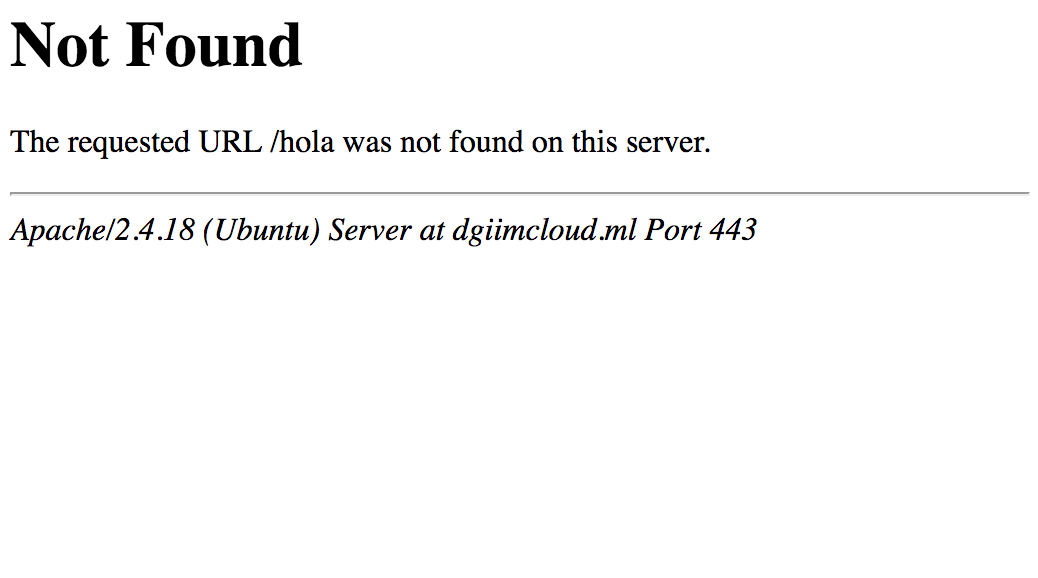
\includegraphics[width=\paperwidth]{404}}
\begin{frame}[plain]
\end{frame}
}

\begin{frame}{Fragilidad}   
  HTTP es frágil porque para acceder al contenido se depende de una serie de servidores concretos.

  Si alguno de ellos falla, no se puede acceder al contenido.
\end{frame}

\begin{frame}{Fragilidad}

  Si un servidor cambia de dirección o deja de estar disponible, los enlaces que apuntan hacia él dejan de funcionar.

  El creador de Pinboard estima que alrededor del 5\% de los enlaces que se almacenan en este servicio dejan de funcionar cada año.

\end{frame}

\begin{frame}{Hipercentralización}
  La web actualmente está altamente centralizada. La práctica totalidad de los usuarios de Internet dependen de una serie de servicios concretos.

  Una caída del servicio de Google en 2013 provocó una reducción mundial del tráfico de Internet del 40\%.
\end{frame}

\begin{frame}{Hipercentralización}
  No hay que irse muy lejos.
\end{frame}

\begin{frame}{Hipercentralización}
  La \textit{hipercentralización} también facilita el control de las comunicaciones de los ciudadanos por parte de los Gobiernos.
\end{frame}

\begin{frame}{Ineficiencia}
  
  ¿Cuál sería el coste aproximado por haber distribuido el vídeo más visto de YouTube?

  (Suponiendo un coste 1 céntimo/GB distribuido y que siempre se reproduce a 720p)

\end{frame}

\begin{frame}{Ineficiencia}
  
  El vídeo en 720p pesa 61,1MB.

  El vídeo se ha reproducido al menos 4.000.000.000 de veces.

  \begin{equation*}
    ((67,1 \cdot 4.000.000.000) \div 1024) \cdot 0,01 = 2\text{.}621\text{.}093,75 \text{€}
  \end{equation*}

\end{frame}

% section problemas_de_http (end)


\section{La web distribuida} % (fold)
\label{sec:la_web_distribuida}

\begin{frame}{¿Qué es?}
  
  La idea de la web distribuida es eliminar la dependencia en una serie de servidores centrales haciendo que cualquier receptor sea a la vez emisor de información.

  Un ejemplo en la naturaleza que ilustra esta idea es la de la ramificación de las neuronas.

\end{frame}

\begin{frame}{Tecnologías de web distribuida}
  
  Blockchain: Ethereum

  Comunicación: BitMessage

  Bases de datos: IPDB

  Web descentralizada: Tor

  Difusión y almacenamiento de información: IPFS

  ...

\end{frame}

% section la_web_distribuida (end)

\section{El protocolo IPFS} % (fold)
\label{sec:el_protocolo_ipfs}

\begin{frame}{¿Qué es?}
  IPFS es un sistema de archivos distribuido.

  Los nodos IPFS se conectan entre sí para transferir datos.

  El protocolo está dividido en un serie de sub-protocolos.
\end{frame}

\begin{frame}[fragile]{Identidades}
  Gestiona la generación y verificación de la identidad de los nodos.

  Cada nodo se identifica por un \texttt{NodeID} que es el \textit{hash} de su clave pública. IPFS no utiliza una función \textit{hash} concreta.

  \begin{lstlisting}[caption={Definición de Nodo.}, language=Golang]
    // Hash criptográfico
    type NodeId Multihash
    type Multihash []byte
    
    // Claves
    type PublicKey []byte
    type PrivateKey []byte

    type Node struct {
      NodeId NodeID
      PubKey PublicKey
      PriKey PrivateKey
    }
  \end{lstlisting}
\end{frame}

\begin{frame}{Red}
  El susbsistema de red de IPFS incluye funciones para:
  \begin{itemize}
    \item Transporte
    \item Fiabilidad
    \item Conectividad
    \item Integridad
    \item Autenticidad
  \end{itemize}
\end{frame}

\begin{frame}{Red}
  IPFS puede utilizar cualquier red: no depende ni asume acceso a IP.
\end{frame}

\begin{frame}[fragile]{Enrutamiento}
  IPFS utiliza una Tabla Hash Distribuida (DSHT).

  \begin{lstlisting}[caption={Interfaz de la DSHT.}, language=Golang]
    type IPFSRouting interface {
      // Obtiene la dirección de un nodo concreto
      FindPeer(node NodeId)

      // Almacena un pequeño dato en la DSHT
      SetValue(key []byte, value []byte)

      // Obtiene un pequeño dato de la DSHT
      GetValue(key []byte)

      // Anuncia que el nodo puede distribuir un dato grande
      ProvideValue(key Multihash)

      // Obtiene una serie de peers distribuyendo un dato grande
      FindValuePeers(key Multihash, min int)
    }
  \end{lstlisting}
\end{frame}

\begin{frame}{Intercambio de bloques: el protocolo BitSwap}
  BitSwap es el protocolo de intercambio de bloques de IPFS. Está inspirado en BitTorrent.

  Los \textit{peers} buscan conseguir un conjunto de bloques (\texttt{want\_list}) y tienen otro conjunto de bloques que ofrecer (\texttt{have\_list}).

  BitSwap actúa como una especie de \textit{mercado}.

  Normalmente el intercambio de archivos no es complementario.
\end{frame}

\begin{frame}{Crédito BitSwap}

  Los nodos envían bloques a sus \textit{peers} de forma optimista.

  Hay que protegerse de los \textit{leeches}.

  Un sistema de créditos resuelve el problema:
  \begin{itemize}
    \item Los \textit{peers} realizan un seguimiento de su saldo con otros nodos.
    \item Los \textit{peers} envían bloques a otros \textit{peers} probabilísticamente.
  \end{itemize}

  Si un nodo decide no enviar bloques a un \textit{peer} el nodo lo ignorará durante un tiempo.

\end{frame}

\begin{frame}{Estrategia BitSwap}
  La elección de una función debe procurar varias cosas.

  Una función que es efectiva en la práctica es una sigmoide, escalada por una \textit{ratio de deuda}.

  \begin{equation*}
    r = \frac{\texttt{bytes\_enviados}}{\texttt{bytes\_recibidos} + 1}
  \end{equation*}

  Dado \textit{r} la probabilidad de enviar a un deudor es:
  \begin{equation*}
    P(r) = 1 - \frac{1}{1 + exp(6-3r)}
  \end{equation*}
\end{frame}

\begin{frame}{Estrategia BitSwap}
  \begin{figure}
  \centering
  \begin{tikzpicture}
    \begin{axis}[
      xlabel=ratio de deuda,
      ylabel={$P(r)$},
      xmin=0,xmax=4,
    ]
    % use TeX as calculator:
    \addplot[accent4,mark=*] {1 - (1/(1 + pow(e, 6-3*x)))};
    \end{axis}
  \end{tikzpicture}
  \caption{Representación de la función de probabilidad $P(r)$.}
\end{figure}
\end{frame}

\begin{frame}[fragile]{Libro mayor de BitSwap}
  Los nodos mantienen un registro de las transferencias con otros nodos.

  Cuando se inicia una conexión entre dos nodos intercambian su libro mayor.

  Si no concuerdan, el libro mayor se destruye. Si la pérdida es intencionada puede que los nodos decidan negar el intercambio de información.

  \begin{lstlisting}[caption={Implementación del libro mayor.}, language=Golang]
  type Ledger struct {
    owner NodeId
    partner NodeId
    bytes_sent int
    bytes_recv int
    timestamp Timestamp
  }
\end{lstlisting}
\end{frame}

\begin{frame}{Conexión BitSwap}

  Esquema de conexión con un \textit{peer}:

  \begin{enumerate}
    \item Conexión: los \textit{peers} envían sus libros mayores hasta que estén de acuerdo.
    \item Envío: los \textit{peers} intercambian sus listas y los bloques.
    \item Cierre: los \textit{peers} desactivan la conexión.
    \item Ignorado: un \textit{peer} es ignorado si el nodo decide no enviar información.
  \end{enumerate}

\end{frame}

\begin{frame}{Grafo Dirigido Acíclico de Merkle}

La implementación del sistema de archivos de IPFS es una generalización de la estructura de datos de Git.

Utilizar un GAD de Merkle nos aporta:

\begin{itemize}
  \item Direccionamiento de contenido
  \item Resistencia a la manipulación
  \item Unicidad
\end{itemize}

\end{frame}

\begin{frame}[fragile]{Rutas}

  Los objetos IPFS pueden ser recorridos con una API de rutas \textit{string} con el siguiente formato:

  \begin{lstlisting}[caption={Rutas en IPFS.}]
  // Formato
  /ipfs/<hash-del-objeto>/<nombre-del-objeto>

  // Ejemplo
  /ipfs/XLYkgq61DYaQ8NhkcqyU7rLcnSa7dSHQ16x/foo.txt
\end{lstlisting}

\end{frame}

\begin{frame}[fragile]{Archivos: \texttt{blob}}

  El objeto \texttt{blob} contiene una unidad de datos direccionable

  Representa un archivo sencillo.

  \begin{lstlisting}[caption={Estructura JSON de un \texttt{blob}.}]
  {
    "data": "datos aquí",
  }
\end{lstlisting}

\end{frame}

\begin{frame}[fragile]{Archivos: \texttt{list}}

  El objeto \texttt{list} representa un archivo grande, formado a partir de varios \texttt{blobs}.

  A diferencia de \texttt{blob}, \texttt{list} tiene enlaces.

  
\begin{lstlisting}[caption={Estructura JSON de un \texttt{list}.}]
  {
    // Las listas pueden tener un array de objetos como datos
    "data": ["blob", "list", "blob"],

    // Las listas no tienen nombres en los enlaces
    "links": [
      { "hash": "nccSbCKcEWHAJ9wj0M72", "size": 38231 },
      { "hash": "2dUB2OS5O7rJBI57n7Hs", "size": 110 },
      { "hash": "BHHGh0pUmwiAyjN5mbTY", "size": 6468 },
    ]
  }
\end{lstlisting}

\end{frame}

\begin{frame}[fragile]{Archivos: \texttt{tree}}

  El objeto \texttt{tree} representa un directorio. Es un \textit{mapeo} de nombres a \textit{hashes}.
  
  \begin{lstlisting}[caption={Estructura JSON de un \texttt{tree}.}]
  {
    // Los árboles pueden tener un array de objetos como datos
    "data": ["blob", "list", "blob"],

    // Las listas no tienen nombres en los enlaces
    "links": [
      { "hash": "nccSbCKcEWHAJ9wj0M72", "name": "test1", "size": 38231 },
      { "hash": "2dUB2OS5O7rJBI57n7Hs", "name": "test2", "size": 110 },
      { "hash": "BHHGh0pUmwiAyjN5mbTY", "name": "test3", "size": 6468 },
    ]
  }
\end{lstlisting}

\end{frame}

\begin{frame}[fragile]{Archivos: \texttt{commit}}

  El objeto \texttt{tree} representa una instantánea en el historial de versiones de cualquier objeto.
  
  \begin{lstlisting}[caption={Estructura JSON de un \texttt{commit}.}]
  {
    "data": {
      "type": "tree",
      "date": "2017-11-12 19:58:00",
      "message": "El mensaje del commit."
    },
    "links": [
      { "hash": "nccSbCKcEWHAJ9wj0M72", "name": "parent", "size": 38231 },
      { "hash": "2dUB2OS5O7rJBI57n7Hs", "name": "object", "size": 110 },
      { "hash": "BHHGh0pUmwiAyjN5mbTY", "name": "author", "size": 6468 },
    ]
  }
\end{lstlisting}

\end{frame}

\begin{frame}{Nomenclatura mutable}
  
  Tal y como hemos descrito hasta ahora IPFS se accede a los archivos por su \textit{hash}.

  Si el contenido del archivo cambia, el \textit{hash} también.

  Necesitamos una forma de acceder a un archivo con una única ruta aunque su contenido cambie.

\end{frame}

\begin{frame}{Nomenclatura mutable: IPNS}
  
  Para ello se define IPNS: InterPlanetary Name Space.

  Asignamos a cada usuario un espacio de nombres mutable en \texttt{ipns/<NodeId>}.

  Se pueden utilizar servicios acortadores de nombres o métodos que permiten codificar una cadena en una serie de palabras fáciles de recordar.

\end{frame}



% section el_protocolo_ipfs (end)

\section{IPFS en la actualidad} % (fold)
\label{sec:la_web_distribuida_en_la_actualidad}

\begin{frame}{Wikipedia descentralizada}
  
  El 29 de abril de 2017 el Gobierno turco bloqueaba el acceso a Wikipedia en el país.

  Pocos días después en el blog oficial de IPFS se anuncia que se ha realizado una instantánea de la Wikipedia turca y que estaba disponible a través de IPFS.

  Actualmente se realizan copias semanales de Wikipedia en Árabe, Inglés, Kurdo y Turco.

\end{frame}

\begin{frame}{Web del referéndum ilegal sobre la independencia de Cataluña (2017)}
  
  La historia del referéndum ya la conocemos todos.

  El Gobierno catalán utilizó IPFS para informar sobre el referéndum y permitir la consulta de los centros de votación.

  Se evita el bloqueo de la web: dominio internacional y contenido distribuido.

\end{frame}

% section la_web_distribuida_en_la_actualidad (end)

\end{document}

